\documentclass{beamer}

\usepackage{beamerthemeIlmenau}
\usepackage{amsthm,amssymb}
\usepackage{mathrsfs}
\usepackage{yfonts}
\usepackage{amsmath,amscd}
\usepackage[mathscr]{euscript}


\usefonttheme[onlymath]{serif}
\usecolortheme{dolphin}
\definecolor{colorTwo}{rgb}{0.86, 0.08, 0.15}
\definecolor{colorPurp}{rgb}{0.45, 0.36, 0.61}

%\setbeamercolor{structure}{fg=colorTwo}

\setbeamercolor{section in head/foot}{bg=colorTwo}
\setbeamercolor{mini frame}{bg=colorTwo}
\setbeamercolor{title}{fg=colorTwo}
\setbeamercolor{frametitle}{fg=colorTwo}


\setbeamercolor{section in head/foot}{fg=black}

\setbeamercolor{subsection in head/foot}{bg=colorPurp}
\setbeamercolor{subsection in head/foot}{fg=black}


%%%%%in header:
\usepackage{tikz}
\usetikzlibrary{matrix}
\usetikzlibrary{arrows} 
\usetikzlibrary{arrows,shapes,shadows}
%%%%%%%%%%%%%

\usepackage{ytableau}
%\usepackage{multicol}

\setbeamertemplate{navigation symbols}{}
\definecolor{pastgrey}{rgb}{0.81, 0.84, 0.78}
\definecolor{spink}{rgb}{0.92, 0.73 , 0.72}
\setbeamercolor{block title}{fg=spink} %color for proof and theorems
\definecolor{PicBlue}{rgb}{0.19, 0.74 , 0.92}

\setbeamercolor{block body}{bg=PicBlue}

\newcommand\T{\rule{0pt}{2.6ex}}
\newcommand\B{\rule[-1.2ex]{0pt}{0pt}}

\newcommand{\C}{\mathbb{C}}
\newcommand{\Q}{\mathbb{Q}}
\newcommand{\R}{\mathbb{R}}
\newcommand{\Z}{\mathbb{Z}}

\newcommand{\sN}{\mathcal{N}}
\newcommand{\sM}{\mathscr{M}}
\newcommand{\sO}{\mathcal{O}}
\newcommand{\sNt}{\widetilde{\mathcal{N}}}
\newcommand{\sMt}{\widetilde{\mathscr{M}}}
\newcommand{\Bx}{\mathscr{B}_x}
\newcommand{\Ox}{\mathcal{O}_G}
\newcommand{\OL}{\mathcal{O}_L}
\newcommand{\Op}{\mathcal{O}_P}
\newcommand{\Mx}{\widetilde{\mathscr{M}}_x}

\newcommand{\Ql}{\mathbb{Q}_{\ell}}
\newcommand{\Qlb}{\overline{\mathbb{Q}}_{\ell}}

\newcommand{\kg}{\mathfrak{g}}
\newcommand{\kh}{\mathfrak{h}}
\newcommand{\kf}{\mathfrak{f}}
\newcommand{\ku}{\mathfrak{u}}
\newcommand{\kb}{\mathfrak{b}}
\newcommand{\kt}{\mathfrak{t}}
\newcommand{\ksl}{\mathfrak{sl}}
\newcommand{\sln}{\mathfrak{sl}_n}

\newcommand{\Tau}{\mathrm{T}}

\newcommand{\IC}{\mathrm{IC}}

\DeclareMathOperator{\Spec}{Spec}
\DeclareMathOperator{\multi}{multi}
\DeclareMathOperator{\Lie}{Lie}
\DeclareMathOperator{\ad}{ad}
\DeclareMathOperator{\rank}{rank}
\DeclareMathOperator{\Irrep}{Irrep}

%\theoremstyle{plain}
\newtheorem{thm}{Theorem}[section]
\newtheorem{cor}[thm]{Corollary}
\newtheorem{lem}[thm]{Lemma}
\newtheorem{prop}[thm]{Proposition}

%\newtheorem{cor}{Corollary}
%\newtheorem*{prop*}{Proposition}

\theoremstyle{definition}
\newtheorem{defn}[thm]{Definition}
\newtheorem{quest}{Question}
\newtheorem{facts}{Facts}
\newtheorem{blank}{}

\renewcommand{\qedsymbol}{$\blacksquare$}

\title{Tile Sets Generated by Hadamard Submatrices of Fourier Matrices}
\author[Troy Wiegand]{Troy Wiegand\\{\footnotesize with faculty mentor Dr. John Herr}}
\date{12 April 2019}
%\institute{University of Georgia}


\begin{document}

\frame{\titlepage}

%\section[Outline]{}
%\frame{\tableofcontents}
\section{Tiling Sets}
\subsection{}
%%%%%%%%%%%%%%%%%%%

\frame{
	\frametitle{What does it mean to tile?}
	Take any finite subset of the integers $A$. \pause \\
	\vspace{.33 in}
	$A$ tiles if there exists some set $T$ such that
	\[ A \oplus T = \mathbb Z \] \pause \\
	$T$ can be decomposed into a finite set of shifts $B$ and a period $N_A$ such that, \[ T=B\oplus N_A \mathbb{Z} .\]


}%%%%%%%%%%%%%%%%%%%%%%%%%%%%%%%%%%%%%%%%%%%%%%%%%%%%%%%%%%%%%%%
\frame{\frametitle{Tiling Example}
	\begin{columns}
		\begin{column}{0.33\textwidth}
			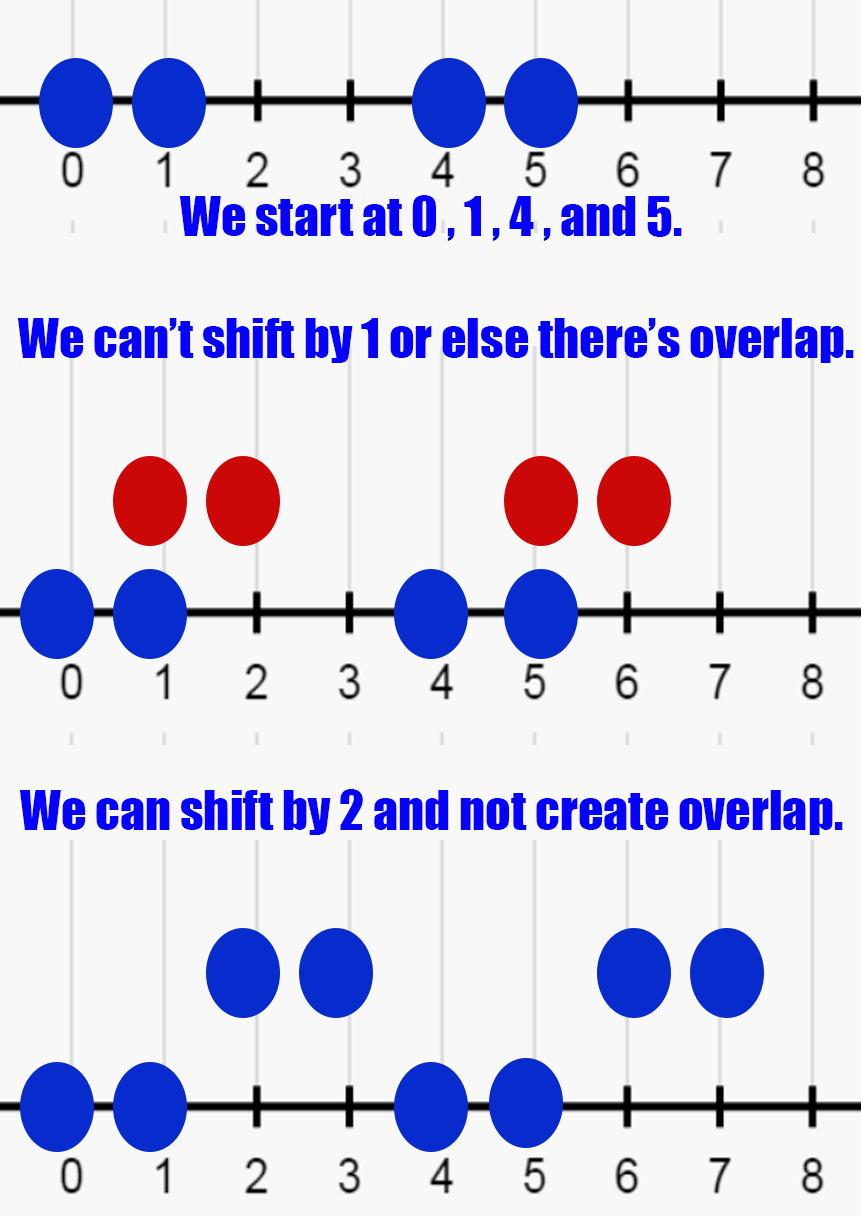
\includegraphics[scale=0.125]{numberline0145.PNG}
		\end{column}

		\begin{column}{0.66\textwidth}
			Let's try to find $T$ for $A=\{ 0,1,4,5 \}$\\
			\pause
			\vspace{.25 in}
			Let start with $B$.
			\pause
			\[ B =  \{0,2 \} \]
			\pause

			Let's try to figure out the $N_A$ of $A$.\\
			\pause
			\[ N_A = 8 \]

		\end{column}

	\end{columns}

	\vspace{.29 in}

	\begin{centering}
		\pause
		Therefore, $T = \{0,2 \} \oplus 8\mathbb Z$.

	\end{centering}

}%%%%%%%%%%%%%%%%%%%%%%%%%%%%%%%%%%%%%%%%%%%%%%%%%%%%%%%%%%%%%%%
\frame{\frametitle{Notation for the CM Properties}

	In 1998 Ethan M. Coven and Aaron Meyerowitz discovered sufficient conditions for a set to tile.\\
	\vspace{0.29 in}
	Here is some more notation that will be necessary to understand the CM Properties:

	\begin{itemize}
		\item $A(x)$ is a polynomial of the form $\sum_{a \in A}x^a$ and $A(1) = |A| $
		\item $S_A$ is the set of prime powers $s$ such that $s$th cyclotomic polynomial $\Phi_s(x) $ divides A(x)
	\end{itemize}

	\vspace{12pt}

}%%%%%%%%%%%%%%%%%%%%%%%%%%%%%%%%%%%%%%%%%%%%%%%%%%%%%%%%%%%%%%%
\frame{\frametitle{CM Properties}


	\begin{thm}
		Given
		\begin{itemize}
			\item[] \textbf{T1} $A(1)$ needs to equal $\prod_{s \in S_A} \Phi_s(1)$
			\item[] \textbf{T2} If $s_1,...,s_m \in S_A$ are powers of distinct primes, then $\Phi_{s_1 \cdot \cdot \cdot s_m }$divides $A(x)$
		\end{itemize}


		\normalsize


		If $|A|$ has at most two prime factors, then $A(x)$ satisfies the two CM Properties (T1 and T2) if and only if $A$ tiles the integers.

	\end{thm}

}%%%%%%%%%%%%%%%%%%%%%%%%%%%%%%%%%%%%%%%%%%%%%%%%%%%%%%%%%%%%%%%
\frame{\frametitle{CM Example}

	\textcolor{colorTwo}{\textbf{Example:} }

	For $A= \{0,1,4,5 \}$, $A(x)=x^5+x^4+x+1$ and $S_A = \{2,8 \}$ \\

	We need to show the two properties in order to show that this set tiles:

	\pause
	\begin{proof}
		\pause
		\begin{itemize}
			\item[] \textbf{T1} $A(1)=(1)^5+(1)^4+(1)+1=4$ and $\prod_{s \in S_A} \Phi_s(1) = (x+1)(x^4+1) |_{x=1} = 4$.  \textbf{T1} is true.
			      \pause
			\item[] \textbf{T2} The numbers $2$ and $8$ are not powers of distinct primes. Thus, \textbf{T2} is true.
		\end{itemize}
		\pause
		Both of our properties are met, therefore this set $A= \{0,1,4,5 \}$ tiles.

	\end{proof}


}%%%%%%%%%%%%%%%%%%%%%%%%%%%%%%%%%%%%%%%%%%%%%%%%%%%%%%%%%%%%%%%
%%%%%%%%%%%%%%%%%%%
\frame{\frametitle{Determining Period and Shifting Set of $A$}


	Coven and Meyerowitz also found that the period and shifting set of $A$ can be determined through use of $A(x)$ and $S_A$.\\

	\[ N_A := lcm(S_A) \]

	\[ B(x) := \prod_{s \in S_B} \Phi_{s}(x^{t(s)}), \]

	where $S_B $ range over the prime power factors of $N_A \not \in S_A$ and $t(s)$ is the largest factor of $N_A$ relatively prime to $s$.\\




}%%%%%%%%%%%%%%%%%%%%%%%%%%%%%%%%%%%%%%%%%%%%%%%%%%%%%%%%%%%%%%%
\frame{\frametitle{Period and Shifting Set Example}


	\textcolor{colorTwo}{\textbf{Example:} }
	Let's look at $A = \{0,1,4,5 \}$ again.\\
	\pause
	Remember $S_A = \{ 2,8 \}$.\\
	\[ N_A = lcm(2,8)=8 .\]
	\pause
	\[ S_B = \{ 4 \} \text{ and } t(4)=\text{largest factor of $N_A$ relatively prime to 4} \]
	\pause
	\[ B(x) = \Phi_{4}(x^{1}) = 1+x^2 \text{\pause \hspace{5pt}  and } B = \{ 0,2 \} .\]

	\pause
	\begin{center}
		Therefore, $T = \{0,2 \} \oplus 8\mathbb Z$.
	\end{center}


}%%%%%%%%%%%%%%%%%%%%%%%%%%%%%%%%%%%%%%%%%%%%%%%%%%%%%%%%%%%%%%%
%%%%%%%%%%%%%%%%%%%
\section{Hadamard and Fourier Matrices}
\subsection{}
%%%%%%%%%%%%%%%%%%%
\frame{
	\frametitle{What is a Hadamard Matrix?}

	A Hadamard Matrix $H$ is a $N$ by $N$ square matrix whose entries all have a complex modulus of one and
	\[ H^{*}H = HH^{*} = N \cdot I_N ,\] where $*$ is the adjoint and $I_N$ is the $N$ by $N$ Identity Matrix.\\

}%%%%%%%%%%%%%%%%%%%%%%%%%%%%%%%%%%%%%%%%%%%%%%%%%%%%%%%%%%%%%%
\frame{\frametitle{What is a Fourier Matrix?}
	Fourier Matrices are a subclass of Hadamard Matrices:\\
	\vspace{.33 in}
	All entries of an $M$ by $M$ Fourier Matrix have the form:
	\[ f_{jk} = e^{2i\pi \frac{(j)(k)}{M}} ,\]
	where $j$ is the $j$th row and $k$ is the $k$th column.
}%%%%%%%%%%%%%%%%%%%%%%%%%%%%%%%%%%%%%%%%%%%%%%%%%%%%%%%%%%%%%%%

\frame{\frametitle{What Am I Doing?}
	Let's look at $\mathcal{F}_4 $.
	\[
		\mathcal{F}_4 =
		\begin{bmatrix}
			1 & 1  & 1  & 1  \\
			1 & i  & -1 & -i \\
			1 & -1 & 1  & -1 \\
			1 & -i & -1 & i
		\end{bmatrix}
	\]
	\pause
	Let's only look at the $0$th and $2$th columns.
	\[
		\begin{bmatrix}
			1 & 1  \\
			1 & -1 \\
			1 & 1  \\
			1 & -1
		\end{bmatrix} \]
}
%%%%%%%%%%%%%%%%%%%%%%%
\frame{\frametitle{What Am I Doing?}
	\[
		\begin{bmatrix}
			1 & 1  \\
			1 & -1 \\
			1 & 1  \\
			1 & -1
		\end{bmatrix} \]

	Let's remove two rows $\{ 2,3 \}$ .\\

	\[
		\begin{bmatrix}
			1 & 1  \\
			1 & -1
		\end{bmatrix}
		\text{ \pause}
		= \mathcal{F}_2 \]

}
%%%%%%%%%%%%%%%%%%%%%%%
%%%%%%%%%%%%%%%%%%%%%%%
\frame{\frametitle{What Am I Doing?}

	\begin{columns}


		\begin{column}{0.32\textwidth}
			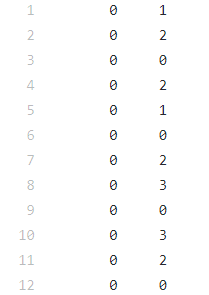
\includegraphics[scale=1]{R4a2input.png}
		\end{column}
		\pause
		\begin{column}{0.68\textwidth}
			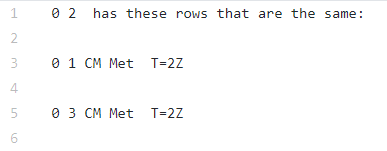
\includegraphics[scale=1]{R4a2output.png}
		\end{column}

	\end{columns}



}
%%%%%%%%%%%%%%%%%%%%%%%
\frame{\frametitle{Why Am I Doing It?}

	\begin{thm}[Universal Tiling Conjecture (Dutkay and Jorgensen, 2013)]
		Let $p \in \mathbb{N}$. Let $\Gamma := {\lambda_0=0, \lambda_1,\lambda_{p-1}}$ be a subset of $\mathbb{R}$ with $p$ elements. Assume $\Gamma$ has a spectrum of the form $\frac{1}{p} A$ with $A \subset \mathbb{Z}$. Then for every finite family $A_1, A_2, ...., A_n$ of subsets of $\mathbb{Z}$ such that $\frac{1}{p} A_i$ is a spectrum for $\Gamma$ for all $i$ there exists a common tiling subset
		$\Tau$ of $\mathbb{Z}$ such that the set $A_i$ tiles $\mathbb{Z}$ by $\Tau$ for all $i \in \{1,....,n\}$.

	\end{thm}


}%%%%%%%%%%%%%%%%%%%%%%%%%%%%%%%%%%%%%%%%%%%%%%%%%%%%%%%%%%%%%%%
%\frame{\frametitle{Fourier Matrix Example}

%\[
%\mathcal{F}_4 =
%\begin{bmatrix}
%e^{2i\pi\frac{0}{4}} & e^{2i\pi\frac{0}{4}} & e^{2i\pi\frac{0}{4}} & e^{2i\pi\frac{0}{4}} \\
%e^{2i\pi\frac{0}{4}} & e^{2i\pi\frac{1}{4}} & e^{2i\pi\frac{2}{4}} & e^{2i\pi\frac{3}{4}} \\
%e^{2i\pi\frac{0}{4}} & e^{2i\pi\frac{2}{4}} & e^{2i\pi\frac{4}{4}} & e^{2i\pi\frac{6}{4}} \\
%e^{2i\pi\frac{0}{4}} & e^{2i\pi\frac{3}{4}} & e^{2i\pi\frac{6}{4}} & e^{2i\pi\frac{9}{4}} 
%\end{bmatrix} =  \begin{bmatrix}
%1 & 1 & 1 & 1 \\
%1 & i & -1 & -i \\
%1 & -1 & 1 & -1 \\
%1 & -i & -1 & i 
%\end{bmatrix} 
%\]  


%}%%%%%%%%%%%%%%%%%%%%%%%%%%%%%%%%%%%%%%%%%%%%%%%%%%%%%%%%%%%%%%%
%\frame{\frametitle{Fuglede Conjecture}
%
%\begin{thm} [Fuglede Conjecture (1974)]
%A domain $\Omega$ admits an operator spectrum if and only if it is possible to %tile $\mathbb{R}^d$ by a family of translates of $\Omega$.
%\end{thm}
%
%\pause
%
%This has been shown to be true in a variety of special cases however it has been %shown to be false in both directions in dimensions 3 and higher. 
%
%	
%}%%%%%%%%%%%%%%%%%%%%%%%%%%%%%%%%%%%%%%%%%%%%%%%%%%%%%%%%%%%%%%%

%\frame{\frametitle{Tying It All Together }
%
%
%
%\begin{thm} [Dutkay and Jorgensen, 2013]
%The following statements are equivalent.
%\begin{enumerate}
%    \item The Universal Tiling Conjecture is true for all $p \in \mathbb{N}$
%    \item Every bounded Lebesgue measurable spectral set tiles by translations.
%\end{enumerate}
%
%Moreover, if these statements are true and if $\Omega, |\Omega |=1, $ is a %bounded Lebesgue measurable set which has a spectrum with period $p$, then $\Omega$ tiles by a subset $\Tau$ of $\frac{1}{p} \mathbb{Z}$
%
%\end{thm}
%
%	
%}%%%%%%%%%%%%%%%%%%%%%%%%%%%%%%%%%%%%%%%%%%%%%%%%%%%%%%%%%%%%%%%

%%%%%%%%%%%%%%%%%%%

%%%%%%%%%%%%%%%%%%%%%%%%%%%%%%%%%%%%%%%%%%%%%%%%%%%%%%%%%%%%%%%%%%
\section{Results/Further Study}
\subsection{}
%%%%%%%%%%%%%%%%%%%

\frame{\frametitle{Results}
	\begin{itemize}
		\item All of the Hadamard submatrices from $\mathcal{F}_{2}$ up to $\mathcal{F}_{18}$ with common columns sets share a common tiling set $T$.

		\item The Hadamard submatrices of size 2, 4, and 5 from $\mathcal{F}_{20}$ with common columns sets share a common tiling set $T$.

		\item  However, there can be multiple tiling sets amongst the same size of Hadamard submatrices generated from the same Fourier Matrix.
	\end{itemize}


}
%%%%%%%%%%%%%%%%%%%%%%%
\frame{\frametitle{Further Study}
	We have developed multiple goals to help guide this project further:
	\begin{itemize}
		\item Write the Hadamard Submatrix Generator in a less interpreted language to be able to gather more submatrices to analyze
		\item Increase the capacity of the Tiling Check Program to handle larger submatrices when they are produced.
	\end{itemize}
}
%%%%%%%%%%%
%%%%%%%%%%%%%%%%%%%%%%%
\frame{\frametitle{References}
	\begin{itemize}
		\item Bond, Bailey, Glickfield, Alexander, and Herr, John E. (2018). On the Existence of Complex Hadamard Submatrices of the Fourier Matrices.
		\item Dutkay, Dorin and Jorgensen, Palle. (2012). On the Universal Tiling Conjecture in Dimension One. Journal of Fourier Analysis and Applications.
		\item Dutkay, Dorin and Kraus, Isabelle. (2018). On spectral sets of integers. Contemporary Mathematics. 215-234.
		\item M. Coven, Ethan and Meyerowitz, Aaron. (1998). Tiling the Integers with Translates of One Finite Set. Journal of Algebra. 212.
		\item Newman, David. (1977). Tesselation of integers. Journal of Number Theory - J NUMBER THEOR.
	\end{itemize}
}

\frame{\frametitle{ }
	\Huge
	\begin{center}
		\textcolor{colorTwo}{\textbf{Any Questions?}}
	\end{center}

}



\end{document}
